\documentclass[border=10pt]{standalone}
\usepackage[svgnames]{xcolor}
\usepackage{amsmath}
\usepackage{pgfplots}
\pgfplotsset{compat=newest}
\usepackage[sfdefault]{FiraSans}
\usepackage{FiraMono}
\renewcommand*\familydefault{\sfdefault}
\begin{document}
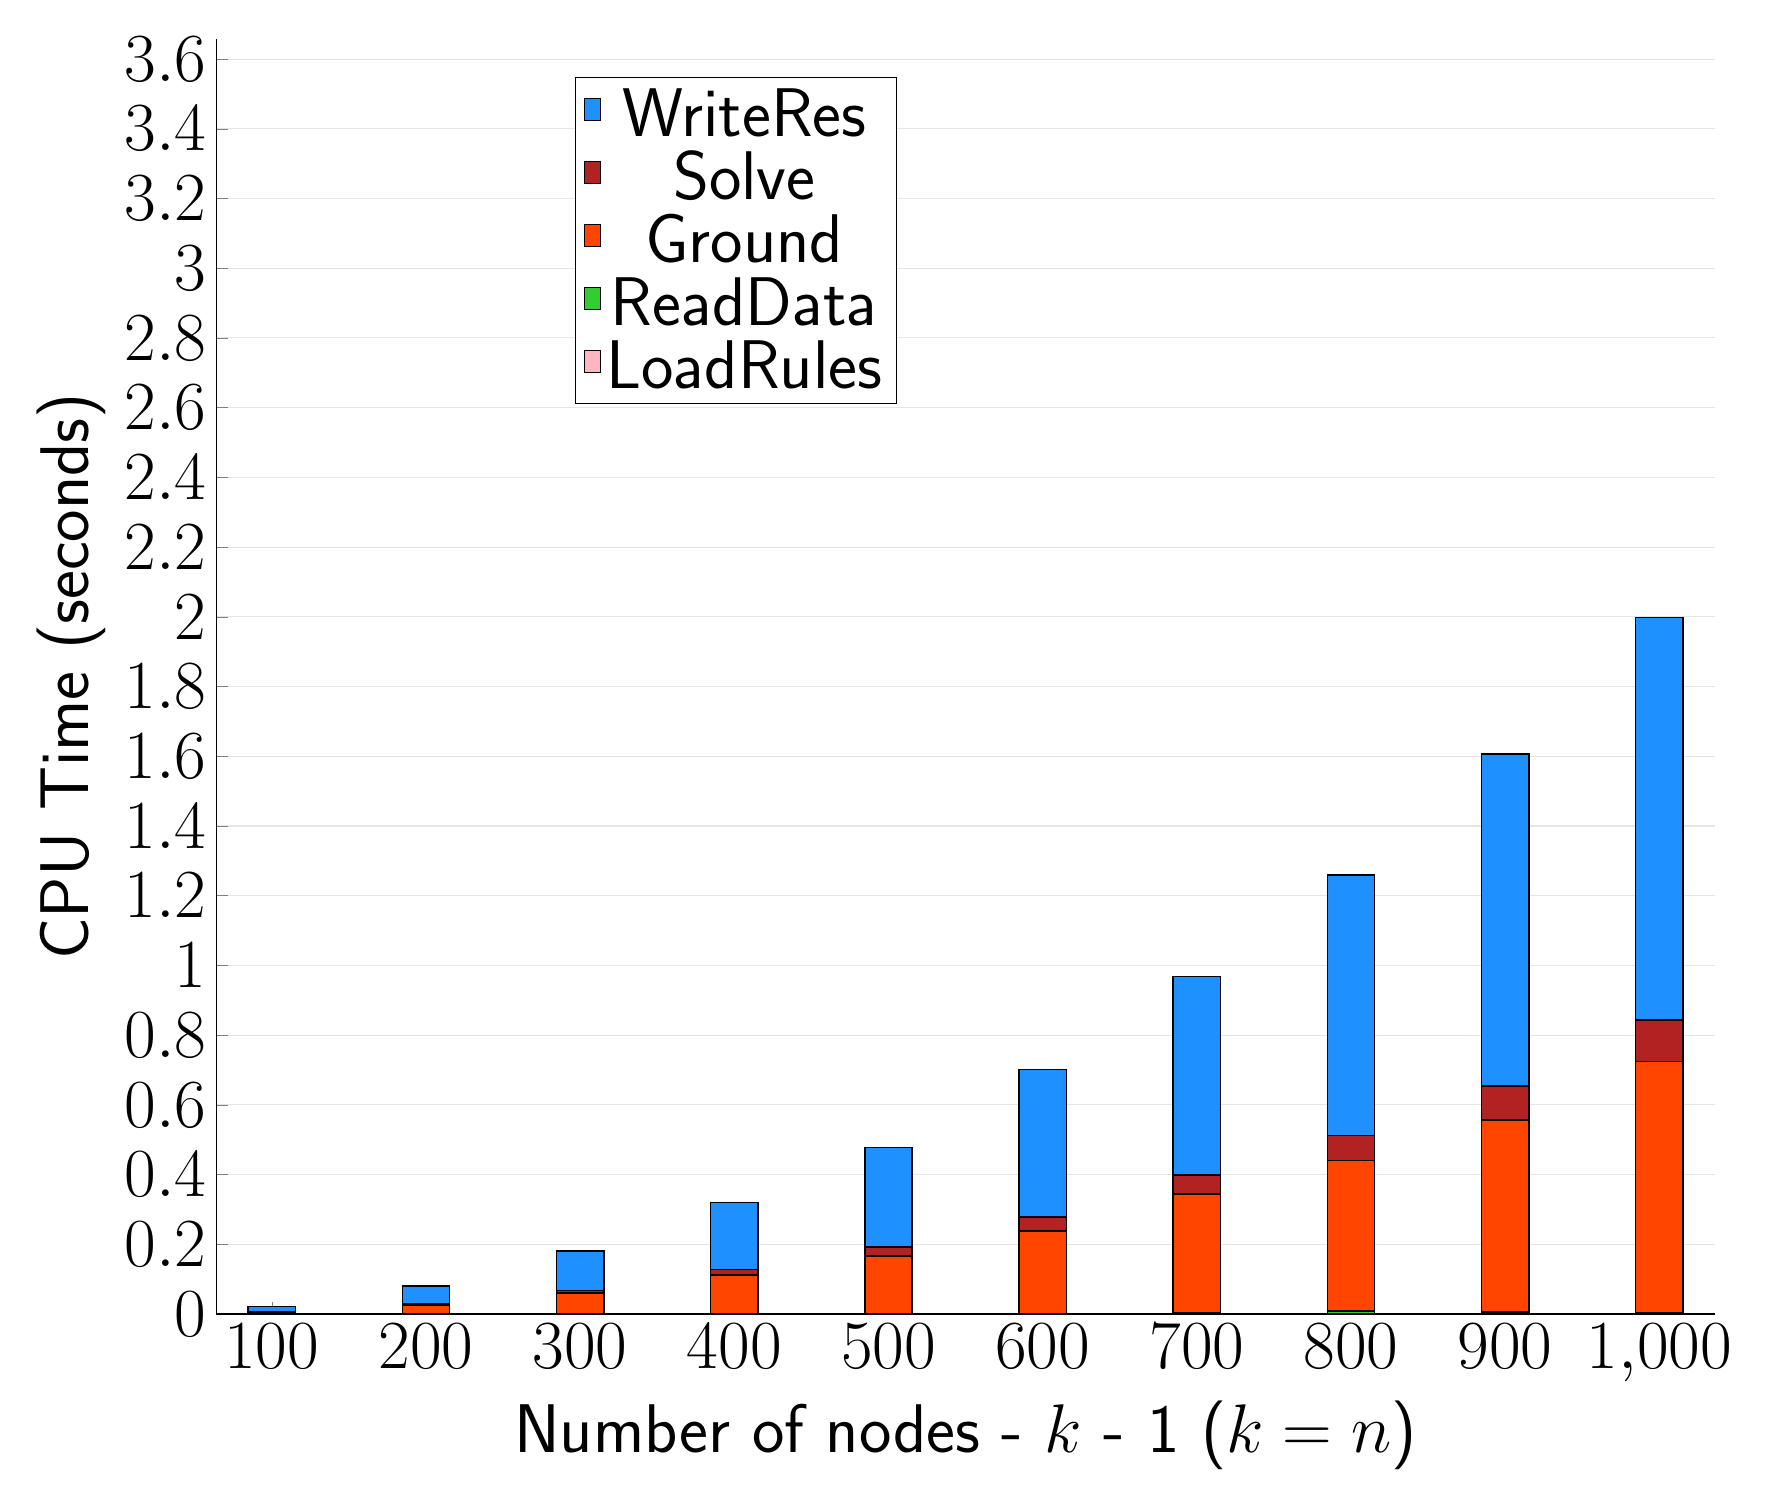
\begin{tikzpicture}
\begin{axis}[
   ybar stacked,
   width=1.7\textwidth,
   bar width=0.6cm,
   ymajorgrids, tick align=inside,
   major grid style={draw=gray!20},
   xtick=data,
   ymin=0, ymax=3.658792,
   axis x line*=bottom,
   axis y line*=left,
   enlarge x limits=0.04,
   legend style={
       at={(0.454, 0.97)},
       anchor=north east,
       legend columns=1,
       font=\Huge,
   },
   ylabel={CPU Time (seconds)},
   xlabel={Number of nodes - $k$ - 1 ($k=n$)},
   label style={font=\Huge},
   tick label style={font=\Huge},
]
\addlegendimage{fill=DodgerBlue, draw=black, line width=0.2pt}
\addlegendentry{WriteRes}
\addlegendimage{fill=FireBrick, draw=black, line width=0.2pt}
\addlegendentry{Solve}
\addlegendimage{fill=OrangeRed, draw=black, line width=0.2pt}
\addlegendentry{Ground}
\addlegendimage{fill=LimeGreen, draw=black, line width=0.2pt}
\addlegendentry{ReadData}
\addlegendimage{fill=LightPink, draw=black, line width=0.2pt}
\addlegendentry{LoadRules}
\addplot +[fill=LightPink, draw=black, line width=0.55pt] coordinates {
(100, 0.0)
(200, 0.0)
(300, 0.0)
(400, 0.0)
(500, 0.0)
(600, 0.001999999999999999)
(700, 0.0)
(800, 0.0)
(900, 0.0)
(1000, 0.0)
};
\addplot +[fill=LimeGreen, draw=black, line width=0.55pt] coordinates {
(100, 0.0)
(200, 0.0)
(300, 0.0019999999999999905)
(400, 0.0)
(500, 0.0020000000000000018)
(600, 0.0)
(700, 0.003999999999999981)
(800, 0.007999999999999962)
(900, 0.005999999999999983)
(1000, 0.003999999999999992)
};
\addplot +[fill=OrangeRed, draw=black, line width=0.55pt] coordinates {
(100, 0.005999999999999994)
(200, 0.026000000000000013)
(300, 0.05800000000000001)
(400, 0.11200000000000002)
(500, 0.16399999999999998)
(600, 0.23600000000000004)
(700, 0.34)
(800, 0.43199999999999994)
(900, 0.55)
(1000, 0.72)
};
\addplot +[fill=FireBrick, draw=black, line width=0.55pt] coordinates {
(100, 0.0)
(200, 0.0040000000000000036)
(300, 0.007999999999999985)
(400, 0.01600000000000001)
(500, 0.026000000000000023)
(600, 0.040000000000000015)
(700, 0.05400000000000005)
(800, 0.07200000000000006)
(900, 0.09800000000000009)
(1000, 0.11999999999999997)
};
\addplot +[fill=DodgerBlue, draw=black, line width=0.55pt] coordinates {
(100, 0.01600000000000001)
(200, 0.04999999999999999)
(300, 0.11200000000000002)
(400, 0.19199999999999995)
(500, 0.28600000000000003)
(600, 0.4239999999999998)
(700, 0.5699999999999998)
(800, 0.7479999999999998)
(900, 0.952)
(1000, 1.1540000000000001)
};
\end{axis}
\end{tikzpicture}

\end{document}
